\documentclass[11pt,a4paper]{article}
\usepackage[utf8]{inputenc}
\usepackage[vietnamese]{babel}
\usepackage{amsmath,amssymb}
\usepackage[version=4]{mhchem}
\usepackage{geometry}
\geometry{top=1.5cm,bottom=1.2cm,left=1.4cm,right=1.4cm,headheight=28pt,headsep=12pt,footskip=18pt}
\usepackage{graphicx}
\usepackage{xcolor}
\usepackage{tabularx}
\usepackage{array}
\usepackage{colortbl}
\usepackage{tikz}
\usepackage{chemfig}
\usepackage{fancyhdr}
\usepackage{enumitem}
\usepackage{multido}
\usepackage{tcolorbox}

\definecolor{hfRed}{HTML}{D32F2F}
\definecolor{hfGreen}{HTML}{8BC390}
\definecolor{mainGreen}{HTML}{2E7D32}
\definecolor{solBlue}{HTML}{1565C0}
\definecolor{tableGreen}{HTML}{E8F5E9}

\usepackage{ex_test}

\pagestyle{fancy}
\fancyhf{}
\renewcommand{\headrulewidth}{0.75pt}
\renewcommand{\headrule}{\hbox to\headwidth{\color{hfGreen}\leaders\hrule height \headrulewidth\hfill}}
\renewcommand{\footrulewidth}{0.75pt}
\renewcommand{\footrule}{\hbox to\headwidth{\color{hfGreen}\leaders\hrule height \footrulewidth\hfill}}

\fancyhead[L]{\small\itshape\color{hfRed}Tài liệu lưu hành nội bộ}
\fancyhead[R]{\small\color{hfRed}Thầy \textbf{TRẦN VĂN THẠNH} - 0777.470.803}

\fancyfoot[L]{\footnotesize\itshape\color{hfRed}CS1: 6/15 Nguyễn Hoàng, P. Kim Long, TP Huế \quad|\quad CS2: 24 Đặng Thái Thân, TP Huế}
\fancyfoot[R]{\small\textbf{\color{hfRed}Trang \thepage}}

\setlength{\parindent}{0pt}
\setlength{\parskip}{2pt}

\begin{document}

\begin{minipage}[t]{0.48\textwidth}
\textbf{SỞ GD\&ĐT THÀNH PHỐ HUẾ}\\
\textbf{TRƯỜNG THPT BÙI THỊ XUÂN}\\
\textit{ĐỀ CHÍNH THỨC}\\
\textit{(Đề thi có 03 trang)}
\end{minipage}
\hfill
\begin{minipage}[t]{0.48\textwidth}
\raggedleft
\textbf{\color{hfRed}KIỂM TRA ĐÁNH GIÁ CUỐI KÌ I}\\
\textbf{NĂM HỌC 2025 -- 2026}\\
\textbf{MÔN: HOÁ HỌC LỚP 11}\\
\textit{Thời gian làm bài: 45 phút (không kể thời gian phát đề)}\\
\textbf{MÃ ĐỀ: 1102}
\end{minipage}

\vspace{4pt}
\noindent
\textit{Họ và tên:} \dotfill \textit{Số báo danh:} \dotfill

\vspace{3pt}
\noindent
\textit{\footnotesize Cho biết nguyên tử khối của các nguyên tố: $\ce{H} = 1; \ce{O} = 16; \ce{C} = 12; \ce{N} = 14; \ce{Na} = 23; \ce{Mg} = 24; \ce{K} = 39; \ce{S} = 32$.}

\vspace{3pt}
\hrule color{hfGreen} height 0.5pt

\vspace{4pt}
\noindent
{\color{mainGreen}\textbf{\Large A. PHẦN TRẮC NGHIỆM (7 điểm)}}

\vspace{3pt}
\noindent
{\color{mainGreen}\textbf{\large PHẦN I. Câu trắc nghiệm nhiều phương án lựa chọn.}}\\
\textit{\small Thí sinh trả lời từ câu 1 đến câu 12. Mỗi câu hỏi thí sinh chỉ chọn một phương án.}
\vspace{2pt}

\begin{ex}
Cho các phát biểu sau:
\begin{enumerate}[label=(\arabic*),leftmargin=1.5cm,itemsep=0pt]
\item Sulfur vừa có tính oxi hóa vừa có tính khử.
\item Trong tự nhiên, sulfur chỉ tồn tại ở dạng hợp chất.
\item $\ce{SO2}$ là acidic oxide, tan trong nước tạo dung dịch có tính acid.
\item $\ce{H2SO4}$ đặc có tính háo nước mạnh và tính oxi hóa mạnh.
\item Trong hợp chất, nguyên tố sulfur có số oxi hóa phổ biến là $-2; +4; +6$.
\end{enumerate}
Số phát biểu đúng là
\choice
{2.}
{3.}
{\True 4.}
{5.}
\end{ex}
\begin{ex}
Dung dịch $\ce{H2SO4}$ loãng có thể tác dụng với cả hai chất nào sau đây?
\choice
{\True $\ce{Fe}$ và $\ce{Fe(OH)3}$.}
{$\ce{S}$ và $\ce{H2S}$.}
{$\ce{C}$ và $\ce{CO2}$.}
{$\ce{Cu}$ và $\ce{Cu(OH)2}$.}
\end{ex}
\begin{ex}
Cặp chất nào sau đây có thể là đồng đẳng của nhau?
\choice
{$\ce{C2H4, C3H8}$.}
{$\ce{CH4O, C2H4O}$.}
{$\ce{CH4, C2H4}$.}
{\True $\ce{C2H2, C4H6}$.}
\end{ex}
\begin{ex}
Để tách tinh dầu sả (có trong thân, lá, rễ .... cây sả) trong công nghiệp hương liệu, người ta dùng phương pháp
\choice
{kết tinh dầu sả trong nước.}
{\True chưng cất bằng hơi nước và chiết tinh dầu ra khỏi hỗn hợp sản phẩm.}
{chưng cất bằng hơi nước và chiết bằng nước lạnh.}
{chiết tinh dầu sả sau đó chưng cất bằng hơi nước.}
\end{ex}
\begin{ex}
Yếu tố không làm ảnh hưởng đến chuyển dịch cân bằng là
\choice
{nồng độ.}
{nhiệt độ.}
{áp suất.}
{\True chất xúc tác.}
\end{ex}
\begin{ex}
Liên kết hoá học trong phân tử $\ce{NH3}$ là liên kết
\choice
{kim loại.}
{\True cộng hoá trị có cực.}
{ion.}
{cộng hoá trị không cực.}
\end{ex}
\begin{ex}
Phổ khối lượng của hợp chất hữu cơ $\ce{X}$ thu được như hình vẽ:
\begin{center}
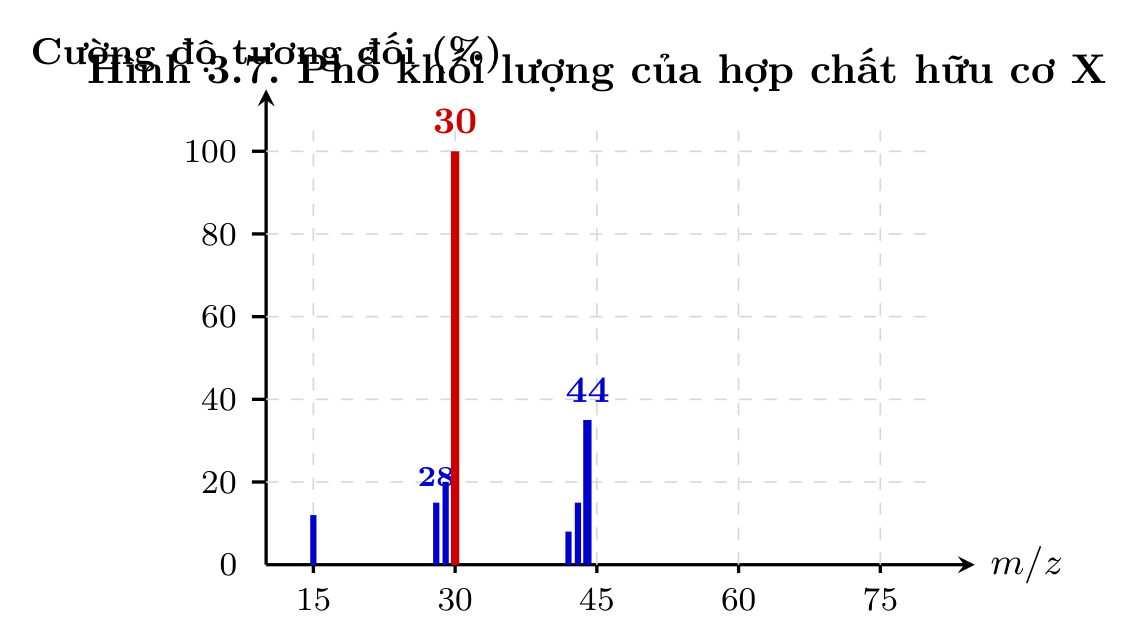
\includegraphics[width=0.48\textwidth]{images_ck1_hoa11_buithixuan/ms_cau7_hd.png}
\end{center}
Phân tử khối của hợp chất hữu cơ $\ce{X}$ là
\choice
{28.}
{75.}
{\True 44.}
{30.}
\end{ex}
\begin{ex}
Chọn phát biểu không đúng?
\choice
{\True Nitrogen là nguyên tố phổ biến nhất trong vỏ trái đất.}
{Nitrogen lỏng được dùng để bảo quản mẫu vật phẩm trong y học.}
{Hai nguyên tử $\ce{N}$ trong phân tử nitrogen liên kết với nhau bằng liên kết ba.}
{Ở nhiệt độ thường, nitrogen khá trơ về mặt hoá học.}
\end{ex}
\begin{ex}
Khí $\ce{NO_x}$ là một trong các nguyên nhân gây nên hiện tượng mưa acid, mù quang hóa, hiện tượng phú dưỡng,... làm ô nhiễm môi trường. Nguồn phát sinh $\ce{NO_x}$ có nguồn gốc tự nhiên là
\choice
{hoạt động giao thông vận tải.}
{\True hoạt động của núi lửa.}
{hoạt động đốt nhiên liệu.}
{hoạt động của nhà máy nhiệt điện.}
\end{ex}
\begin{ex}
Trong các phát biểu sau đây, phát biểu nào đúng khi một hệ ở trạng thái cân bằng?
\choice
{Phản ứng nghịch đã dừng.}
{\True Nồng độ của các chất trong hệ không đổi.}
{Nồng độ chất tham gia và sản phẩm bằng nhau.}
{Phản ứng thuận đã dừng.}
\end{ex}
\begin{ex}
Để xác định nồng độ mol của một dung dịch $\ce{NaOH}$, người ta đã tiến hành chuẩn độ bằng dung dịch $\ce{HCl}$ 0,1M. Để chuẩn độ 10 mL dung dịch $\ce{NaOH}$ này cần 12 mL dung dịch $\ce{HCl}$. Nồng độ của dung dịch $\ce{NaOH}$ trên là
\choice
{0,012M.}
{\True 0,12M.}
{0,1M.}
{1,2M.}
\end{ex}
\begin{ex}
Liên kết hoá học chủ yếu trong phân tử hợp chất hữu cơ là
\choice
{liên kết ion.}
{liên kết cho-nhận.}
{\True liên kết cộng hoá trị.}
{liên kết hydrogen.}
\end{ex}
\vspace{4pt}
\noindent
{\color{mainGreen}\textbf{\large PHẦN II. Câu trắc nghiệm đúng sai.}}\\
\textit{\small Thí sinh trả lời từ câu 1 đến câu 2. Trong mỗi ý a), b), c), d) ở mỗi câu, thí sinh chọn đúng hoặc sai.}
\vspace{2pt}

\begin{ex}
Sulfur và các hợp chất của nó có vai trò quan trọng trong sản xuất và đời sống, nhưng khí thải và chất thải chứa sulfur nếu không được xử lí đúng cách sẽ gây tác động tiêu cực đến sức khỏe con người và môi trường.
\choiceTF
{\True Ở điều kiện thường, lưu huỳnh là chất rắn, màu vàng, không tan trong nước, tan nhiều trong các dung môi hữu cơ như benzene, carbon disulfide ($\ce{CS2}$)...}
{Khí $\ce{SO2}$ có thể được dùng làm chất tẩy màu, khi hoà tan khí này vào nước tạo ra dung dịch làm quỳ tím hoá xanh.}
{\True Thuốc thử nhận biết sulfuric acid và muối sulfate là ion $\ce{Ba^2+}$ trong $\ce{BaCl2, Ba(OH)2, Ba(NO3)2}$.}
{\True Sulfuric acid đặc lấy nước từ hợp chất carbohydrate và khiến chúng hoá đen chứng tỏ sulfuric acid có tính háo nước.}
\end{ex}
\begin{ex}
Hợp chất hữu cơ $\ce{X}$ được sử dụng rộng rãi trong đời sống như làm dung môi, nhiên liệu sinh học và thành phần chính của đồ uống có cồn. Kết quả phân tích nguyên tố hợp chất $\ce{X}$ cho thấy có 52,17\% carbon, 34,78\% oxygen, còn lại là hydrogen. Tỉ khối hơi của $\ce{X}$ so với khí hydrogen bằng 23. Phổ IR của $\ce{X}$ có dải hấp thụ đặc trưng được mô tả trong hình dưới đây:
\begin{center}
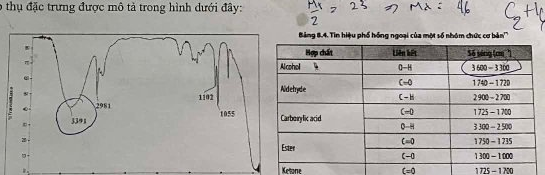
\includegraphics[width=0.72\textwidth]{images_ck1_hoa11_buithixuan/ir_cau2_p2.png}
\end{center}
\choiceTF
{\True Công thức phân tử của $\ce{X}$ là $\ce{C2H6O}$.}
{Do $\ce{X}$ tan vô hạn trong nước và có nhiệt độ sôi thấp hơn nước, nên không thể tách $\ce{X}$ khỏi hỗn hợp với nước bằng phương pháp chưng cất.}
{\True Dựa vào phổ IR, có thể dự đoán phân tử $\ce{X}$ chứa nhóm chức $-\ce{OH}$.}
{Chất $\ce{CH3OCH3}$ không phải là đồng phân cấu tạo của $\ce{X}$.}
\end{ex}
\vspace{4pt}
\noindent
{\color{mainGreen}\textbf{\large PHẦN III. Câu trắc nghiệm trả lời ngắn.}}\\
\textit{\small Thí sinh trả lời từ câu 1 đến câu 4. Thí sinh điền kết quả vào ô trả lời tương ứng.}
\vspace{2pt}

\begin{ex}
Cho cân bằng hóa học: $\ce{N2(g) + O2(g) <=> 2NO(g)} \quad \Delta_r H^\circ_{298} = +180\text{ kJ}$.
Có các biện pháp sau:
(1) Tăng nhiệt độ.
(2) Hạ nhiệt độ.
(3) Tăng nồng độ $\ce{O2}$.
(4) Tăng áp suất chung của hệ phản ứng.
(5) Dùng thêm chất xúc tác $\ce{V2O5}$.\\
Hỏi có bao nhiêu biện pháp làm cân bằng trên chuyển dịch?

\noindent\textit{Trả lời:} \dotfill
\end{ex}
\begin{ex}
Cho các chất sau: $\ce{HCOOH, CaCO3, C2H4, CO, C6H12O6, NaCN}$. Số chất thuộc loại hợp chất hữu cơ là bao nhiêu?

\noindent\textit{Trả lời:} \dotfill
\end{ex}
\begin{ex}
Các bước tách một hợp chất hữu cơ bằng phương pháp chiết được mô tả như sau:
\begin{enumerate}[label=(\arabic*),leftmargin=1.5cm,itemsep=0pt]
\item Để yên phễu chiết cho hai lớp chất lỏng phân tách hoàn toàn.
\item Lắc nhẹ phễu chiết để chất cần tách chuyển sang dung môi chiết.
\item Cho hỗn hợp chất lỏng không trộn lẫn vào phễu chiết cùng dung môi thích hợp.
\item Mở khóa phễu chiết để thu từng lớp chất lỏng riêng biệt.
\end{enumerate}
Hãy sắp xếp các bước trên theo đúng thứ tự thực hiện của phương pháp chiết.

\noindent\textit{Trả lời:} \dotfill
\end{ex}
\begin{ex}
Geraniol là một hợp chất hữu cơ tự nhiên có mùi hoa hồng đặc trưng, được sử dụng rộng rãi trong sản xuất nước hoa, mỹ phẩm và hương liệu thực phẩm; công thức cấu tạo của geraniol được biểu diễn như sau:
\begin{center}
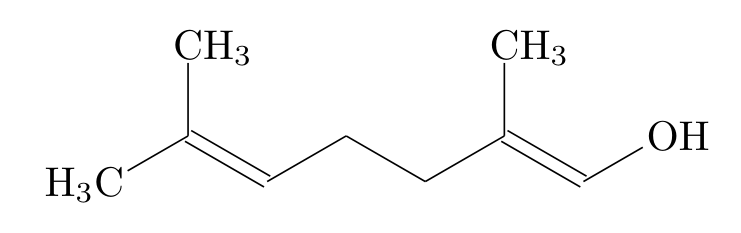
\includegraphics[width=0.45\textwidth]{images_ck1_hoa11_buithixuan/geraniol_hd.png}
\end{center}
Số nguyên tử hydrogen có trong phân tử geraniol là bao nhiêu?

\noindent\textit{Trả lời:} \dotfill
\end{ex}
\vspace{6pt}
\noindent
{\color{mainGreen}\textbf{\Large B. PHẦN TỰ LUẬN (3,0 điểm)}}
\vspace{2pt}

\noindent
\textbf{Câu 1: (0,5 điểm)} Cho $0,04\text{ mol }\ce{Mg}$ tan hết trong dung dịch $\ce{HNO3}$ thấy thoát ra $0,01\text{ mol}$ khí $\ce{X}$ là sản phẩm khử duy nhất (đkc). Xác định công thức của khí $\ce{X}$?

\vspace{1pt}
\noindent
\multido{\n=1+1}{5}{\dotfill\\[4pt]}

\vspace{4pt}
\noindent
\textbf{Câu 2: (1,0 điểm)} Bằng phương pháp hoá học hãy nhận biết các dung dịch sau: $\ce{NaCl, (NH4)2SO4}$ và $\ce{NH4Cl}$. Viết các phương trình phản ứng xảy ra.

\vspace{1pt}
\noindent
\multido{\n=1+1}{7}{\dotfill\\[4pt]}

\vspace{4pt}
\noindent
\textbf{Câu 3: (1,0 điểm)} Acetic acid được sử dụng rộng rãi trên thế giới trong nhiều ngành công nghiệp khác nhau như tạo ra polymer ứng dụng trong sơn, chất kết dính, là dung môi hoà tan các chất hoá học, sản xuất và bảo quản thực phẩm, đặc biệt dùng để sản xuất giấm.\\
a) Lập công thức phân tử của acetic acid, biết kết quả phân tích nguyên tố acetic acid có 40\% C; 53,33\% O về khối lượng; còn lại là H. Phân tử khối của acetic acid được xác định trên phổ khối lượng tương ứng với peak có giá trị $m/z$ lớn nhất.\\
\begin{center}
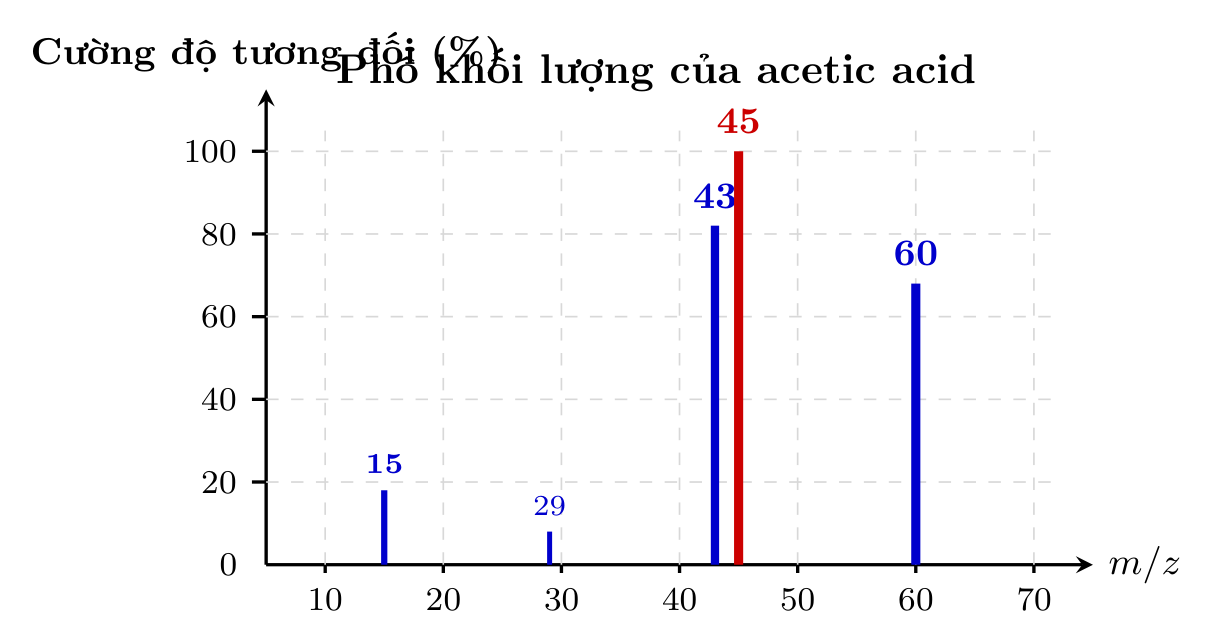
\includegraphics[width=0.48\textwidth]{images_ck1_hoa11_buithixuan/ms_acetic_acid_hd.png}
\end{center}
b) Theo khuyến cáo an toàn, lượng acetic acid trong thực phẩm không nên vượt quá 10 gam trên mỗi một kg thực phẩm. Một cơ sở chế biến thực phẩm dùng 50 mL giấm ăn 5\% để tạo vị chua cho 1,0 kg dưa muối. Biết khối lượng riêng của giấm ăn bằng $1,00\text{ g/mL}$. Hỏi lượng acetic acid sử dụng có vượt quá giới hạn an toàn hay không, giải thích?

\vspace{1pt}
\noindent
\multido{\n=1+1}{8}{\dotfill\\[4pt]}

\vspace{4pt}
\noindent
\textbf{Câu 4: (0,5 điểm)} Hãy viết các đồng phân mạch hở có cùng công thức phân tử $\ce{C2H7N}$?

\vspace{1pt}
\noindent
\multido{\n=1+1}{5}{\dotfill\\[4pt]}

\vspace{6pt}
\begin{center}
\textbf{\large ---------- HẾT ----------}
\end{center}

\end{document}
